\par Dans le but de comparer les modèles basés sur des réseaux de neurones artificiels que l'on entraîne à d'autres modèles prédictifs d'apprentissage automatique, nous entraînons deux modèles de régression linéaire à effectuer les mêmes tâches. Ces modèles sont une régression d'arête (\emph{ridge regression}) avec l'astuce du noyau (\emph{kernel trick}), et une machine à vecteur de support (SVM). Nous utilisons pour cela les implémentations fournies par la bibliothèque Scikit-Learn\cite{sklearn}. L'implémentation de ces deux modèles est identique, à la différence que le modèle \emph{Kernel Ridge Regression} (KRR) utilise le carré des erreurs comme fonction de coût, alors que le modèle SVM utilise une fonction $\epsilon$-insensible, c'est à dire que les erreurs coûtent leur valeur brute, ou valent zéro si elles sont inférieures à un seuil $\epsilon$ donné.
\\

\subsection{Données d'entrée et complexité algorithmique}

\par Afin d'avoir une idée des performances relatives de tous ces modèles, nous les entraînons à prédire les distances relatives entre des atomes de carbone formant une liaison. Ces modèles sont équivalents au modèle \emph{DIST\_REL\_C\_05} (REF DIST REL C 05), car on applique une restriction aux atomes les plus proches de la liaison, et on limite la largeur des entrées à 15 atomes. Ce choix de données d'entrée est lié à la nécessité de fournir des entrées de petite taille (comparativement aux données que l'on donne aux réseaux de neurones) à ces modèles, qui ont une complexité d'entraînement augmentant très vite avec le nombre et la taille des exemples. Avec $n$ le nombre d'exemples et $m$ leur largeur, la complexité de l'entraînement d'un modèle SVM varie entre $O(n^2\times m)$ et $O(n^3\times m)$. La complexité de l'entraînement des modèles KRR n'est pas disponible dans la documentation de Scikit-Learn, mais elle plus grande encore que celle des SVM.
\par Pour la même raison, le nombre d'exemples dans les jeux d'entraînement de ces modèles est beaucoup plus faible que celui des jeux utilisés pour entraîner les réseaux de neurones artificiels. Les modèles que l'on décrit dans cette partie s'entraînent sur des jeux contenant 60000 exemples, ce qui représente tout de même environ cinq jours de temps CPU pour l'entraînement d'un modèle KRR.
\par Enfin, la fonction inverse est appliquée aux distances dans les données d'entrée de ces modèles. En effet, si les réseaux de neurones artificiels sont capables d'approximer ces fonctions, ce n'est pas le cas des modèles que l'on entraîne ici. L'application de la fonction inverse permet de donner des coefficients aux modèles exprimant l'influence des atomes au voisinage des liaisons en fonction de leur distance.

\subsection{Entraînement de modèles KRR}

\subsubsection{Recherche par quadrillage des paramètres}
Afin d'entraîner un modèle fournissant de bons résultats, nous commençons par effectuer une recherche par quadrillage avec trois validations croisées des paramètres pour le modèle KRR. Cette recherche est effectuée sur la grille de paramètres suivante. Selon la documentation, une valeur faible du paramètre alpha va diminuer la variance des erreurs. Le degré correspond au degré du polynôme, et le paramètre coef0 correspond au coefficient constant du polynôme. Les résultats de la recherche par quadrillage sont donnés en annexe (REF ANNEXES QUADRI KER RIDGE).

\begin{figure}[!h]
	\centering
	
	\begin{tabular}{|l|l|}
		\hline
		\textbf{Paramètres} & \textbf{Valeurs} \\ \hline 
		Noyau (\emph{kernel}) & linéaire\\ \hline
		Alpha & 0.1, 0.01, 0.001 \\ \hline
	\end{tabular}
	
	\vspace{0.5cm}	

	\begin{tabular}{|l|l|}
		\hline
		\textbf{Paramètres} & \textbf{Valeurs} \\ \hline 
		Noyau (\emph{kernel}) & polynomial\\ \hline
		Degré & 2, 6 \\ \hline
		Alpha & 0.1, 0.01, 0.001 \\ \hline
		Coef0 & 1, 0.5, 2 \\ \hline
	\end{tabular}		
	
	\caption{Grille de recherche par quadrillage des paramètres pour les modèles KRR}
\end{figure}

\subsubsection{Entraînement d'un modèle et analyse des prédictions}
\par À l'issue de la recherche par quadrillage, on utilise les meilleurs paramètres pour entraîner un modèle KRR (\emph{DIST\_REL\_C\_KER\_RIDGE\_01}) sur les 60000 exemples de notre jeu d'entraînement. Les paramètres sont donnés dans le tableau suivant.

\begin{figure}[!h]
	\centering
	\begin{tabular}{|l|l|}
		\hline
		\textbf{Paramètre} & \textbf{Valeur} \\ \hline
		Noyau & polynomial \\ \hline
		Degré & 2 \\ \hline
		Alpha & 0.01 \\ \hline
		Coef0 & 1 \\ \hline
	\end{tabular}		
	\caption{Paramètres d'entraînement du modèle \emph{DIST\_REL\_C\_KER\_RIDGE\_01}}
\end{figure}

\par Les valeurs des métriques évaluant les erreurs sont données dans le tableau suivant. On y voit que le modèle est très performant pour un premier ensemble de paramètres issu d'une petite recherche par quadrillage. L'erreur médiane est en effet de l'ordre du demi picomètre et l'erreur moyenne de l'ordre du picomètre.

\begin{figure}[!h]
	\centering
	\begin{tabular}{|l|r|}
		\hline
		\textbf{Métrique} & \textbf{Valeur} \\ \hline
		Moyenne & 1,0378 \\ \hline
		Médiane & 0,5891 \\ \hline
		Écart-type & 1,2668 \\ \hline
		Minimum & 0,0000 \\ \hline
		Maximum & 21,6264\\ \hline
		Erreur relative moyenne & 0.7057\% \\ \hline
	\end{tabular}
	
	\caption{Analyse statistique des erreurs du modèle \emph{DIST\_REL\_C\_KER\_RIDGE\_01} (en pm)}
\end{figure}

\par La représentation graphique de la distribution des erreurs et des prédictions disponible dans les figures ci-dessous montre que les erreurs au delà de 10 pm sont très minoritaires, mais montre également que le modèle prédit difficilement les distances peu représentées, à la limite entre les différents types de liaisons.
\par Pour résumer, les modèles prédictifs de type KRR semblent permettent d'obtenir des prédictions proches de la précision requise et pourraient donc être utilisés pour prédire la géométrie convergée complète d'une molécule (REF MODULES), notamment dans le cas des liaisons qui sont peu représentées dans les données, et pour lesquelles les modèles prédictifs basés sur des réseaux de neurones artificiels seront probablement moins efficaces.

\begin{figure}[!h]
	\centering
	
	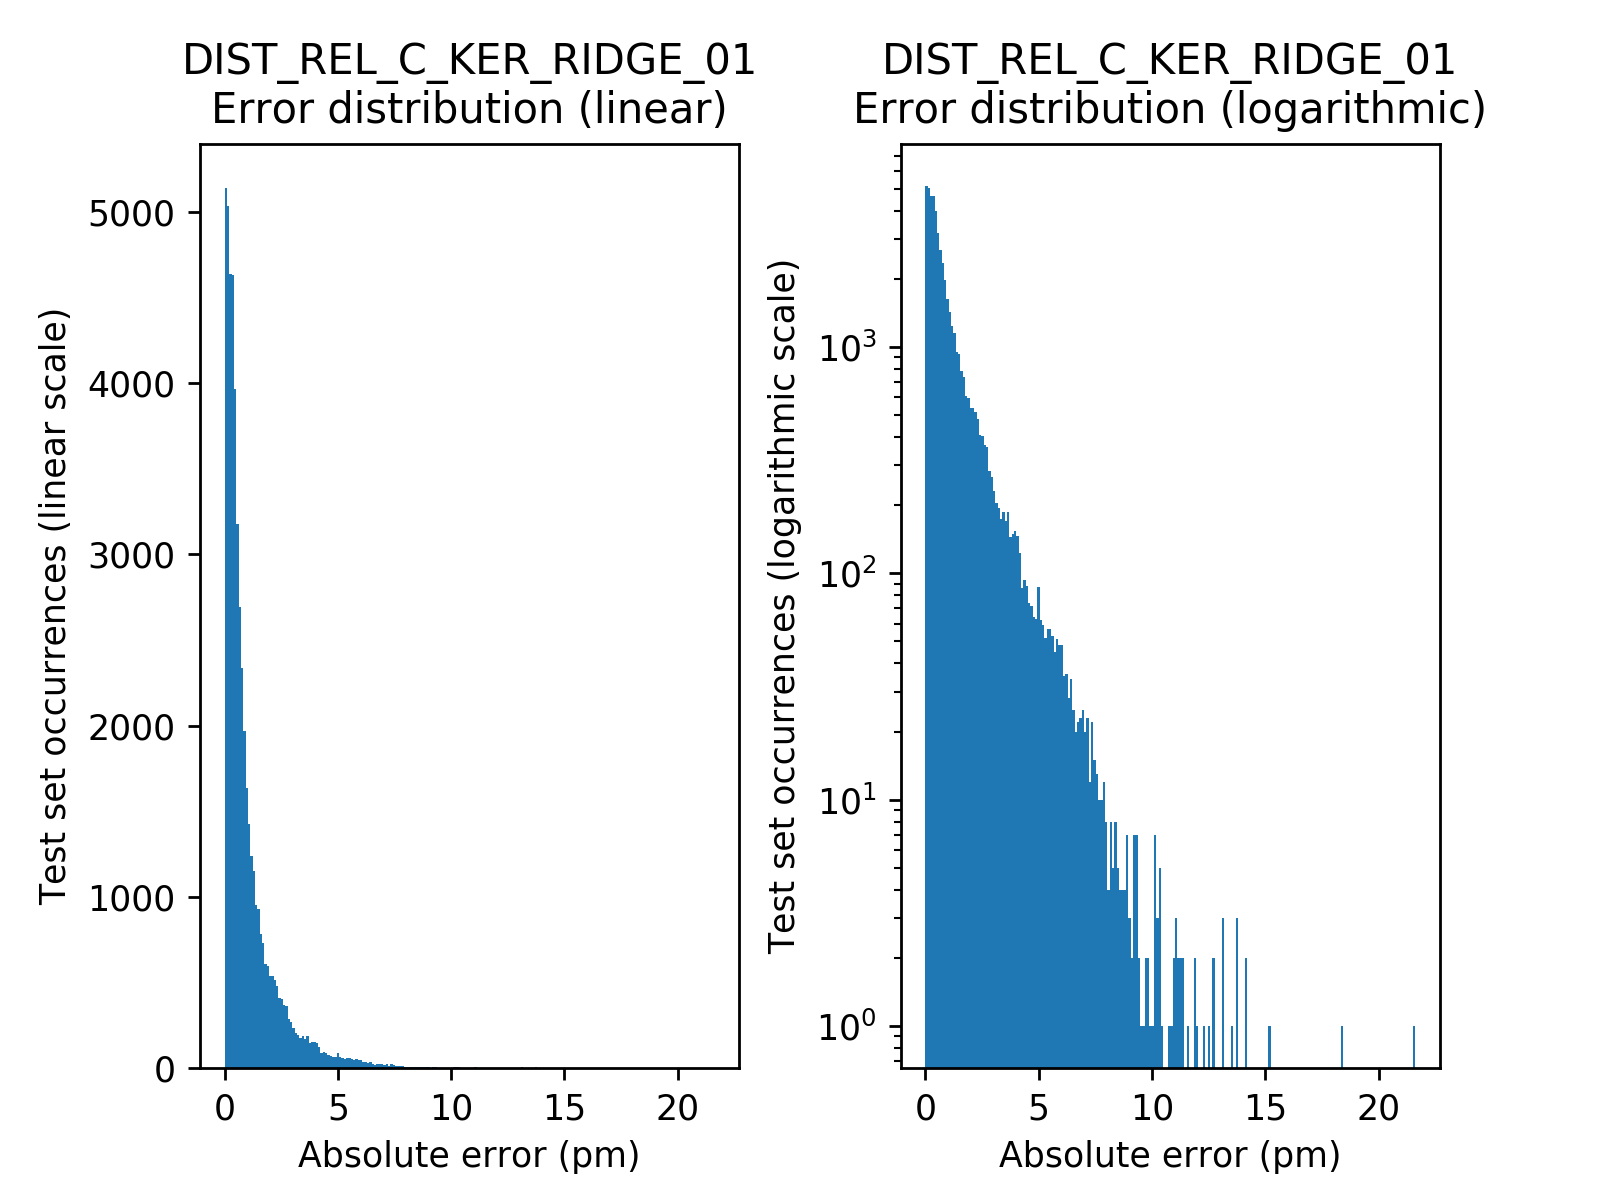
\includegraphics[scale=0.8]{../figures/DIST_REL_C_KER_RIDGE_01/DIST_REL_C_KER_RIDGE_01_distrib_rmse_val.png}	
	
	\caption{Distribution des erreurs du modèle \emph{DIST\_REL\_C\_KER\_RIDGE\_01}}
\end{figure}
\begin{figure}[!h]
	\centering
	
	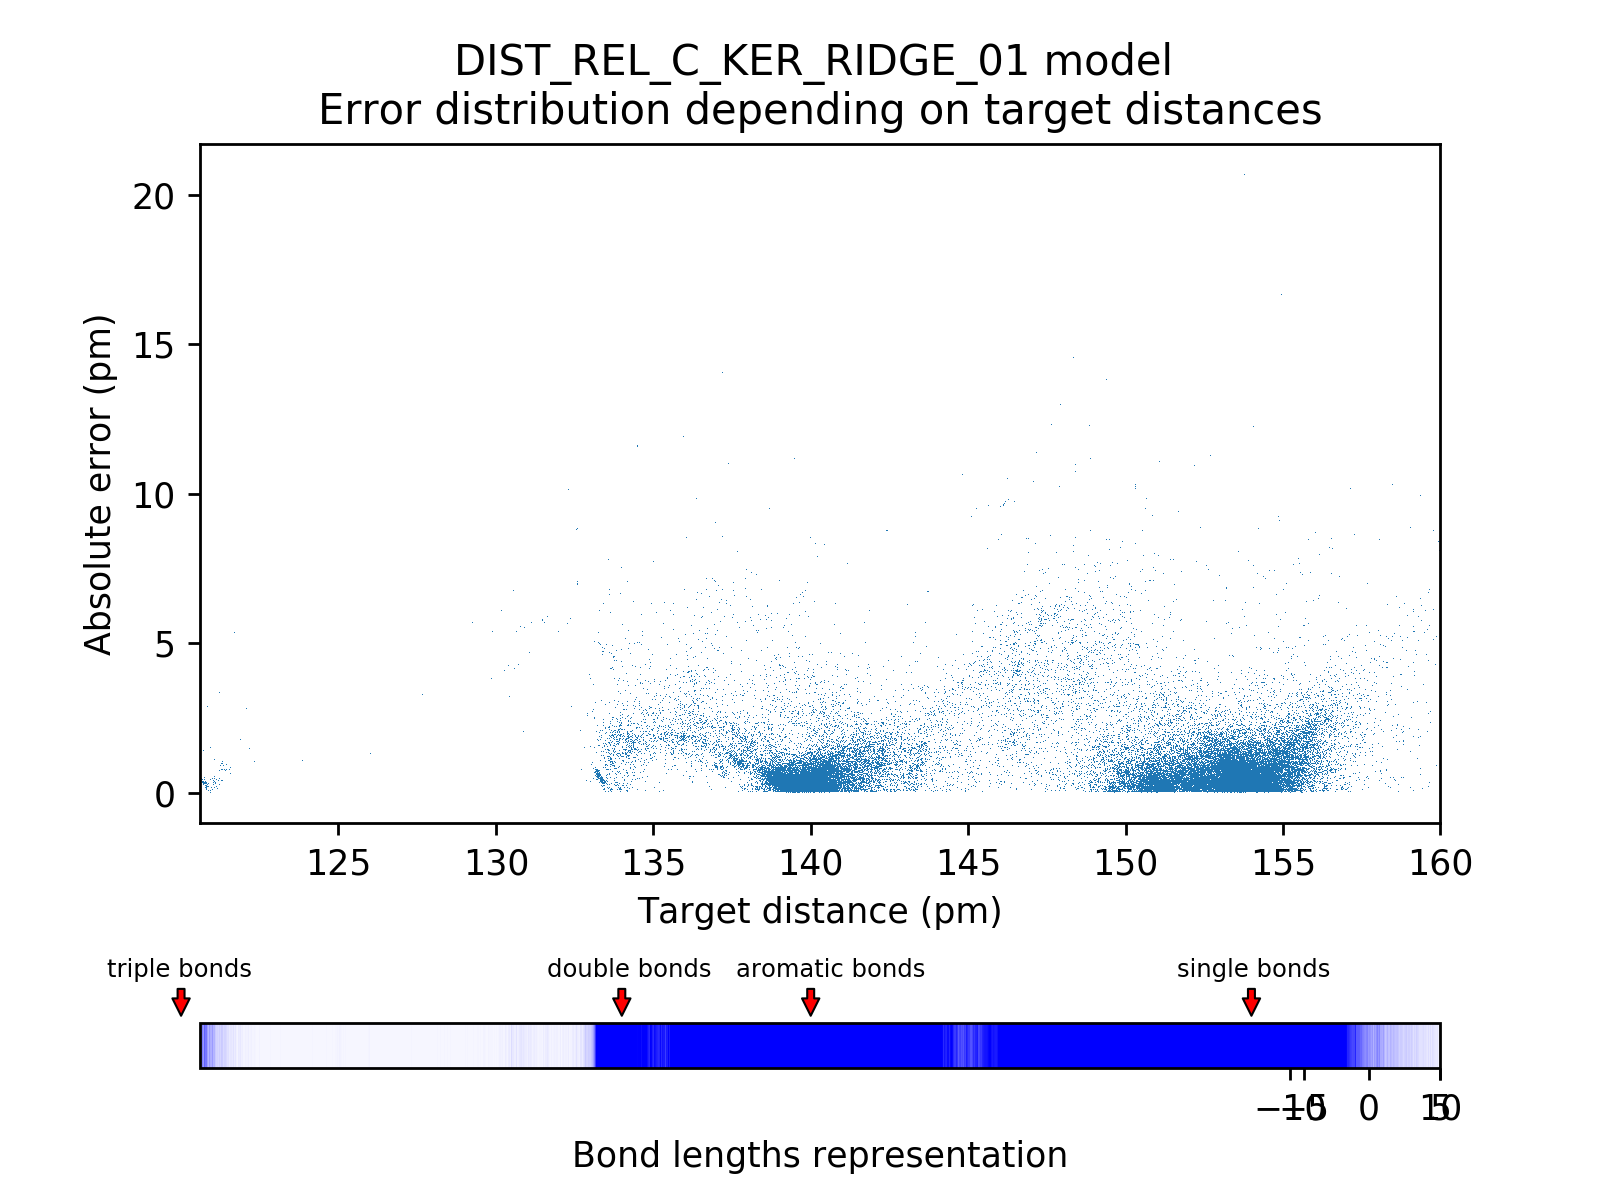
\includegraphics[scale=0.8]{../figures/DIST_REL_C_KER_RIDGE_01/DIST_REL_C_KER_RIDGE_01_distrib_rmse_dist.png}	
	
	\caption{Erreur en fonction des cibles pour le modèle \emph{DIST\_REL\_C\_KER\_RIDGE\_01}}
	\end{figure}

\begin{figure}[!h]
	\centering
	
	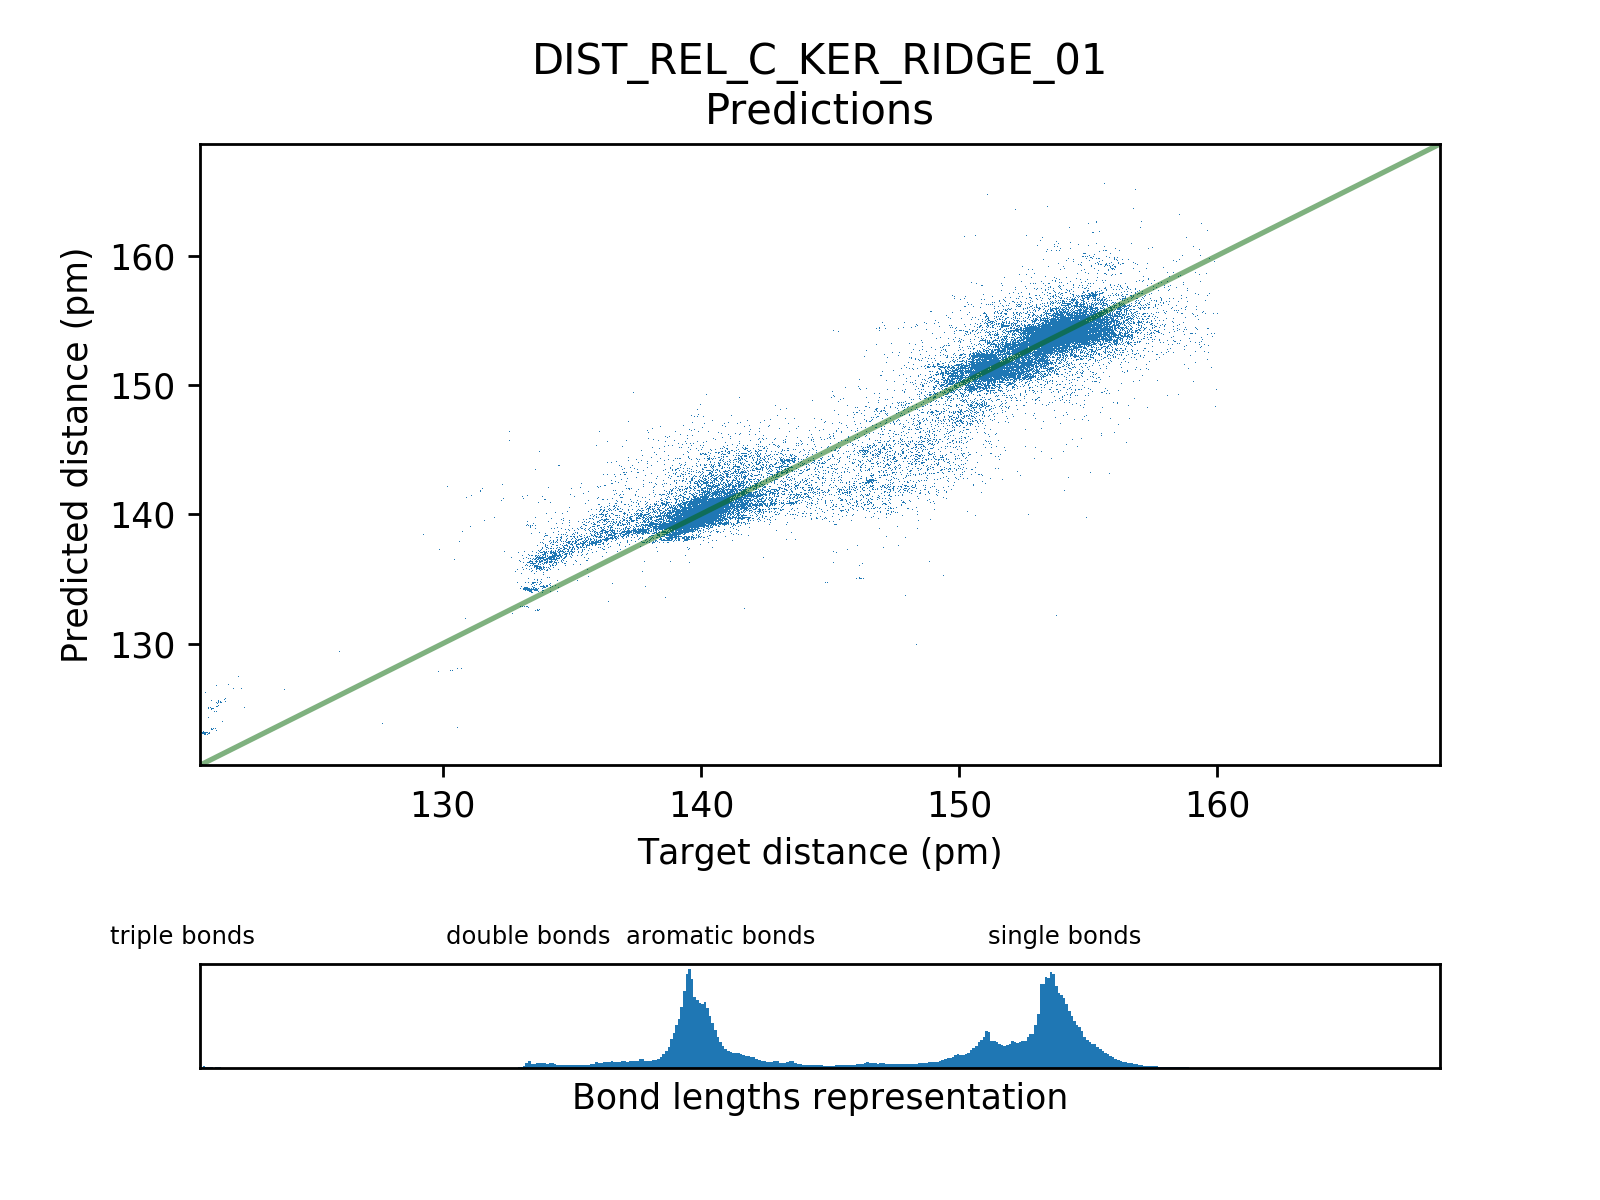
\includegraphics[scale=0.8]{../figures/DIST_REL_C_KER_RIDGE_01/DIST_REL_C_KER_RIDGE_01_preds_targets.png}	
	
	\caption{Prédictions en fonction des cibles pour le modèle \emph{DIST\_REL\_C\_KER\_RIDGE\_01}}
	
\end{figure}

\subsection{Entraînement de modèles SVM}

\subsubsection{Recherche par quadrillage des paramètres (non aboutie)}
Dans l'idée d'appliquer la même méthodologie que pour le modèle de type KRR, nous définissons une grille de recherche par quadrillage des paramètres des modèles SVM. Cette grille est en revanche plus large, puisqu'elle définit l'entraînement de 256 modèles différents avec trois validations croisées, soit l'entraînement de 768 modèles.
La grille de paramètres utilisée est disponible dans la figure ci-dessous. Malheureusement, la recherche n'a pas abouti car certains ensembles de paramètres menaient à l'entraînement de modèles en un temps non raisonnable. Parmi les modèles de la grille, 747 ont été entraînés en environ deux minutes, tandis que l'entraînement des 21 restants n'était pas terminé au bout d'une dizaine d'heures, ce qui a mené à l'interruption de la recherche.

\begin{figure}[!h]
	\centering
	
	\begin{tabular}{|l|l|}
		\hline
		\textbf{Paramètres} & \textbf{Valeurs} \\ \hline 
		Noyau (\emph{kernel}) & linéaire\\ \hline
		$\epsilon$ (fonction de coût) & 0.1, 0.001 \\ \hline
		Coef0 & 0, 0.1, 0.5, 1 \\ \hline
		Heuristique de rétrécissement (\emph{Shrinking}) & True, False \\ \hline
		Tolérance de l'arrêt de l'optimisation & 0.001, 0.01 \\ \hline
		Pénalité sur le terme d'erreur (C) & 1, 0.01\\ \hline
	\end{tabular}
	
	\vspace{0.5cm}	

	\begin{tabular}{|l|l|}
		\hline
		\textbf{Paramètres} & \textbf{Valeurs} \\ \hline 
		Noyau (\emph{kernel}) & polynomial\\ \hline
		$\epsilon$ (fonction de coût) & 0.1, 0.001 \\ \hline
		Gamma (coefficient utilisé par le noyau) & auto, 0.001, 0.01 \\ \hline
		Coef0 & 0, 0.1, 0.5, 1 \\ \hline
		Heuristique de rétrécissement (\emph{Shrinking}) & True, False \\ \hline
		Tolérance de l'arrêt de l'optimisation & 0.001, 0.01 \\ \hline
		Pénalité sur le terme d'erreur (C) & 1, 0.01\\ \hline
	\end{tabular}		
	
	\caption{Grille de recherche par quadrillage des paramètres pour les modèles SVM}
\end{figure}

\subsubsection{Entraînement d'un modèle et analyse des prédictions}
\par La recherche par quadrillage des paramètres n'ayant pas abouti, nous utilisons les paramètres issus de la recherche par quadrillage pour le modèle de type KRR, dans l'idée qu'ils devraient permettre également d'obtenir de bons résultats, et nous laissons les autres paramètres à leur valeur par défaut. Les statistiques des erreur du modèle alors entraîné sont donné dans le tableau suivant. Notons que le fait que le numéro chronologique du modèle soit « 03 » est la conséquence de l'entraînement de deux modèles préalables dont le but était d'estimer le temps d'entraînement en fonction de la taille des données d'entrée.\\

\begin{figure}[!h]
	\centering
	\begin{tabular}{|l|r|}
		\hline
		\textbf{Métrique} & \textbf{Valeur} \\ \hline
		Moyenne & 1,2854 \\ \hline
		Médiane & 0,5005 \\ \hline
		Écart-type & 2,2301 \\ \hline
		Minimum & 0,0000 \\ \hline
		Maximum & 24,2225\\ \hline
		Erreur relative moyenne & 0.8907\% \\ \hline
	\end{tabular}
	
	\caption{Analyse statistique des erreurs du modèle \emph{DIST\_REL\_C\_SVM\_03} (en pm)}
\end{figure}

\par Les statistiques comme les figures suivantes représentant graphiquement les erreurs et les prédictions du modèle disponibles montrent que ses résultats sont nettement inférieurs aux modèles précédents. Le modèle se contente en effet de prédire des valeurs de l'ordre des deux types de liaisons les plus représentées, et ne prédit pas correctement les longueurs de liaisons de tailles intermédiaires.\\


\begin{figure}[!h]
	\centering
	
	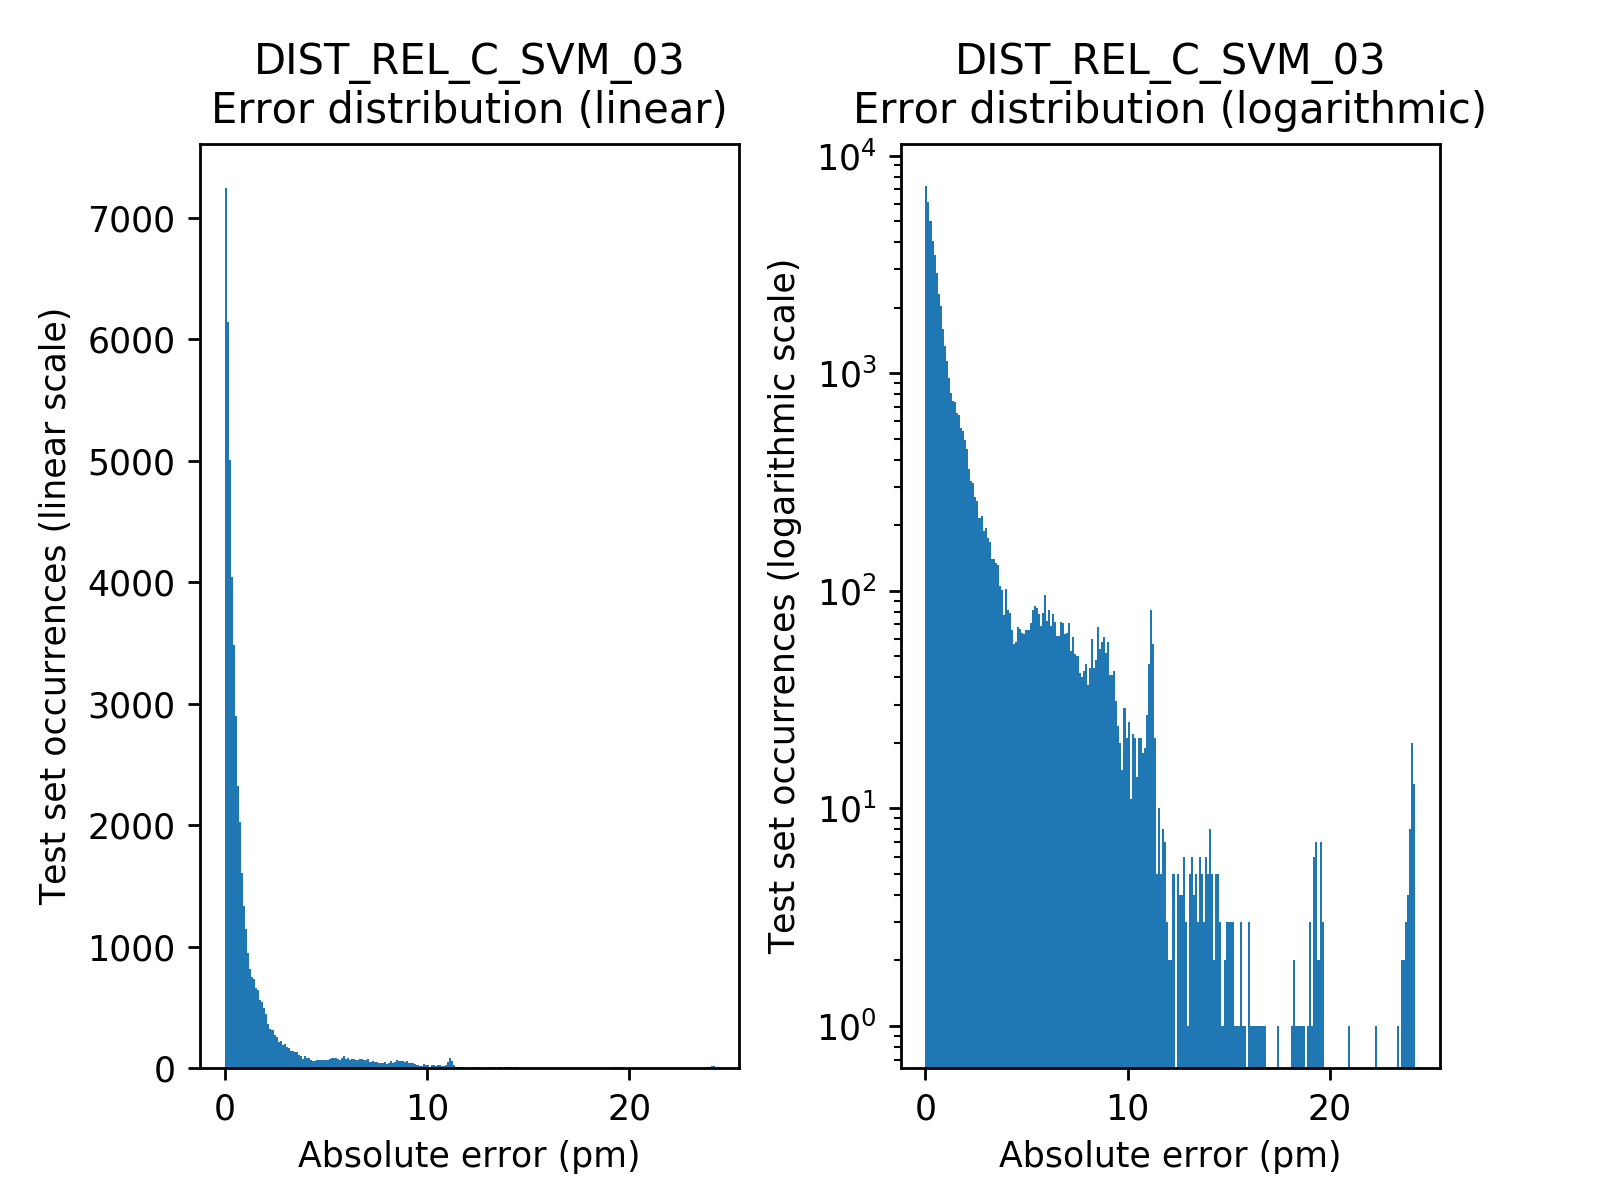
\includegraphics[scale=0.8]{../figures/DIST_REL_C_SVM_03/DIST_REL_C_SVM_03_distrib_rmse_val.png}	
	
	\caption{Distribution des erreurs du modèle \emph{DIST\_REL\_C\_SVM\_03}}
\end{figure}
\begin{figure}[!h]
	\centering
	
	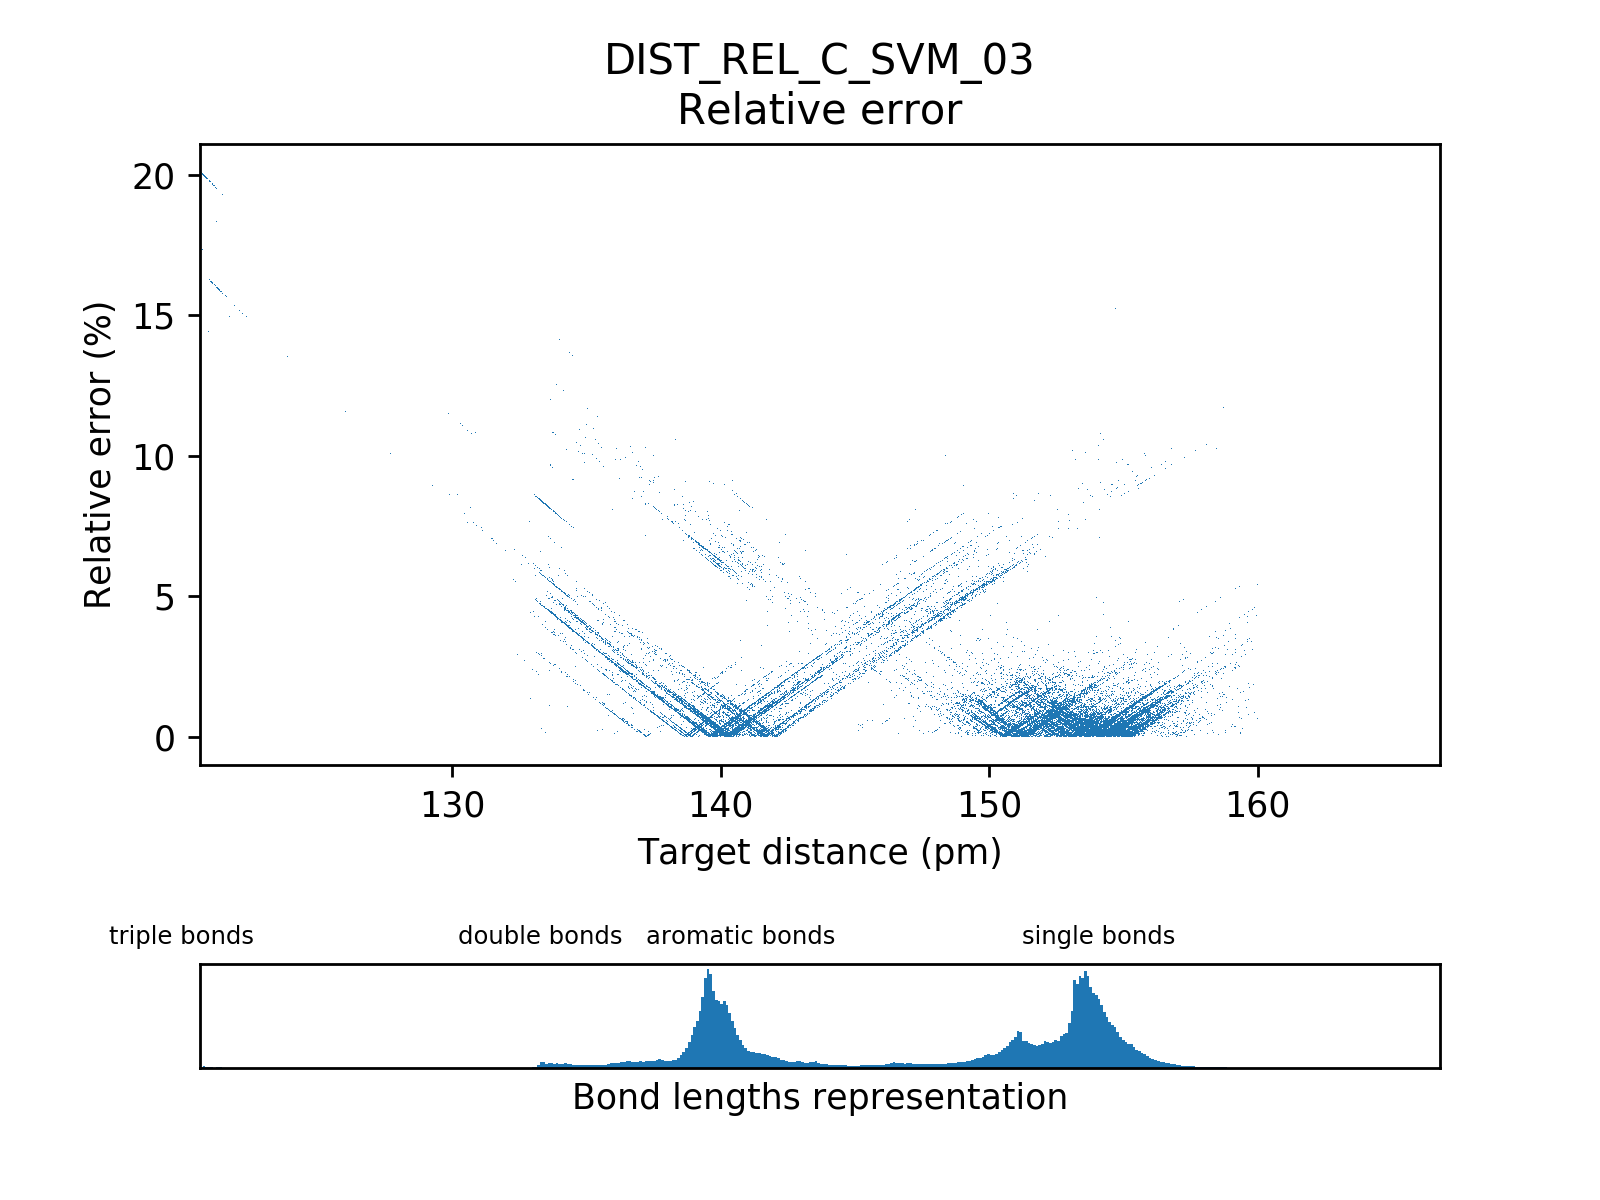
\includegraphics[scale=0.8]{../figures/DIST_REL_C_SVM_03/DIST_REL_C_SVM_03_distrib_rmse_dist.png}	
	
	\caption{Erreur en fonction des cibles pour le modèle \emph{DIST\_REL\_C\_SVM\_03}}
	\end{figure}

\begin{figure}[!h]
	\centering
	
	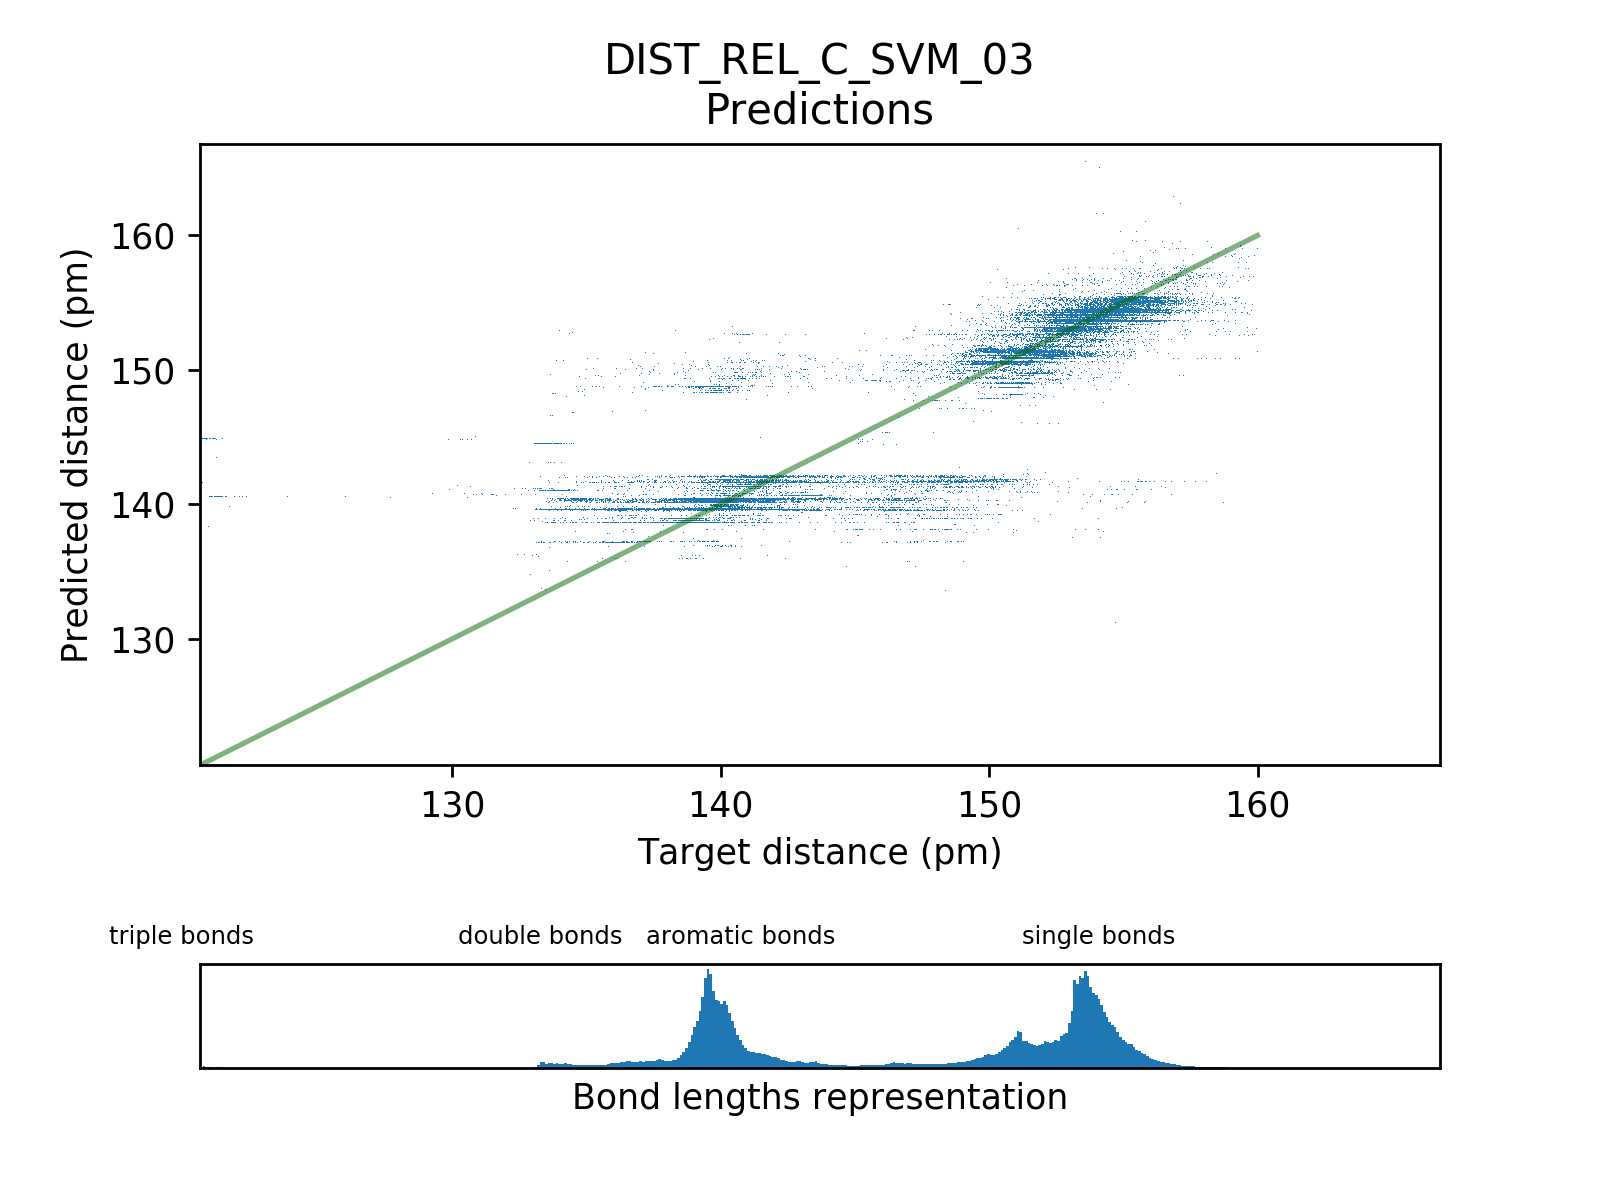
\includegraphics[scale=0.8]{../figures/DIST_REL_C_SVM_03/DIST_REL_C_SVM_03_preds_targets.png}	
	
	\caption{Prédictions en fonction des cibles pour le modèle \emph{DIST\_REL\_C\_SVM\_03}}
	
\end{figure}

